\section{Methods and Materials}
% Here you should describe the design of your solution, your
% technical decisions, and why you believe your solution is appropriate. Some general
% images are recommended to enhance your explanation, and this section is expected
% to be 1 to 2 pages long. It is not recommended to include code here, but if you are
% presenting a complex algorithm, you may add it. Remember to write full paragraphs,
% with one idea per paragraph, and avoid using itemized lists. Aim for clarity and
% readability.

Our desing first of all we make a component diagram to show the components of our system,
and how they are related to each other. The diagram is shown in Fig. \ref{fig:component_diagram}.
\begin{figure}[h]
    \centering
    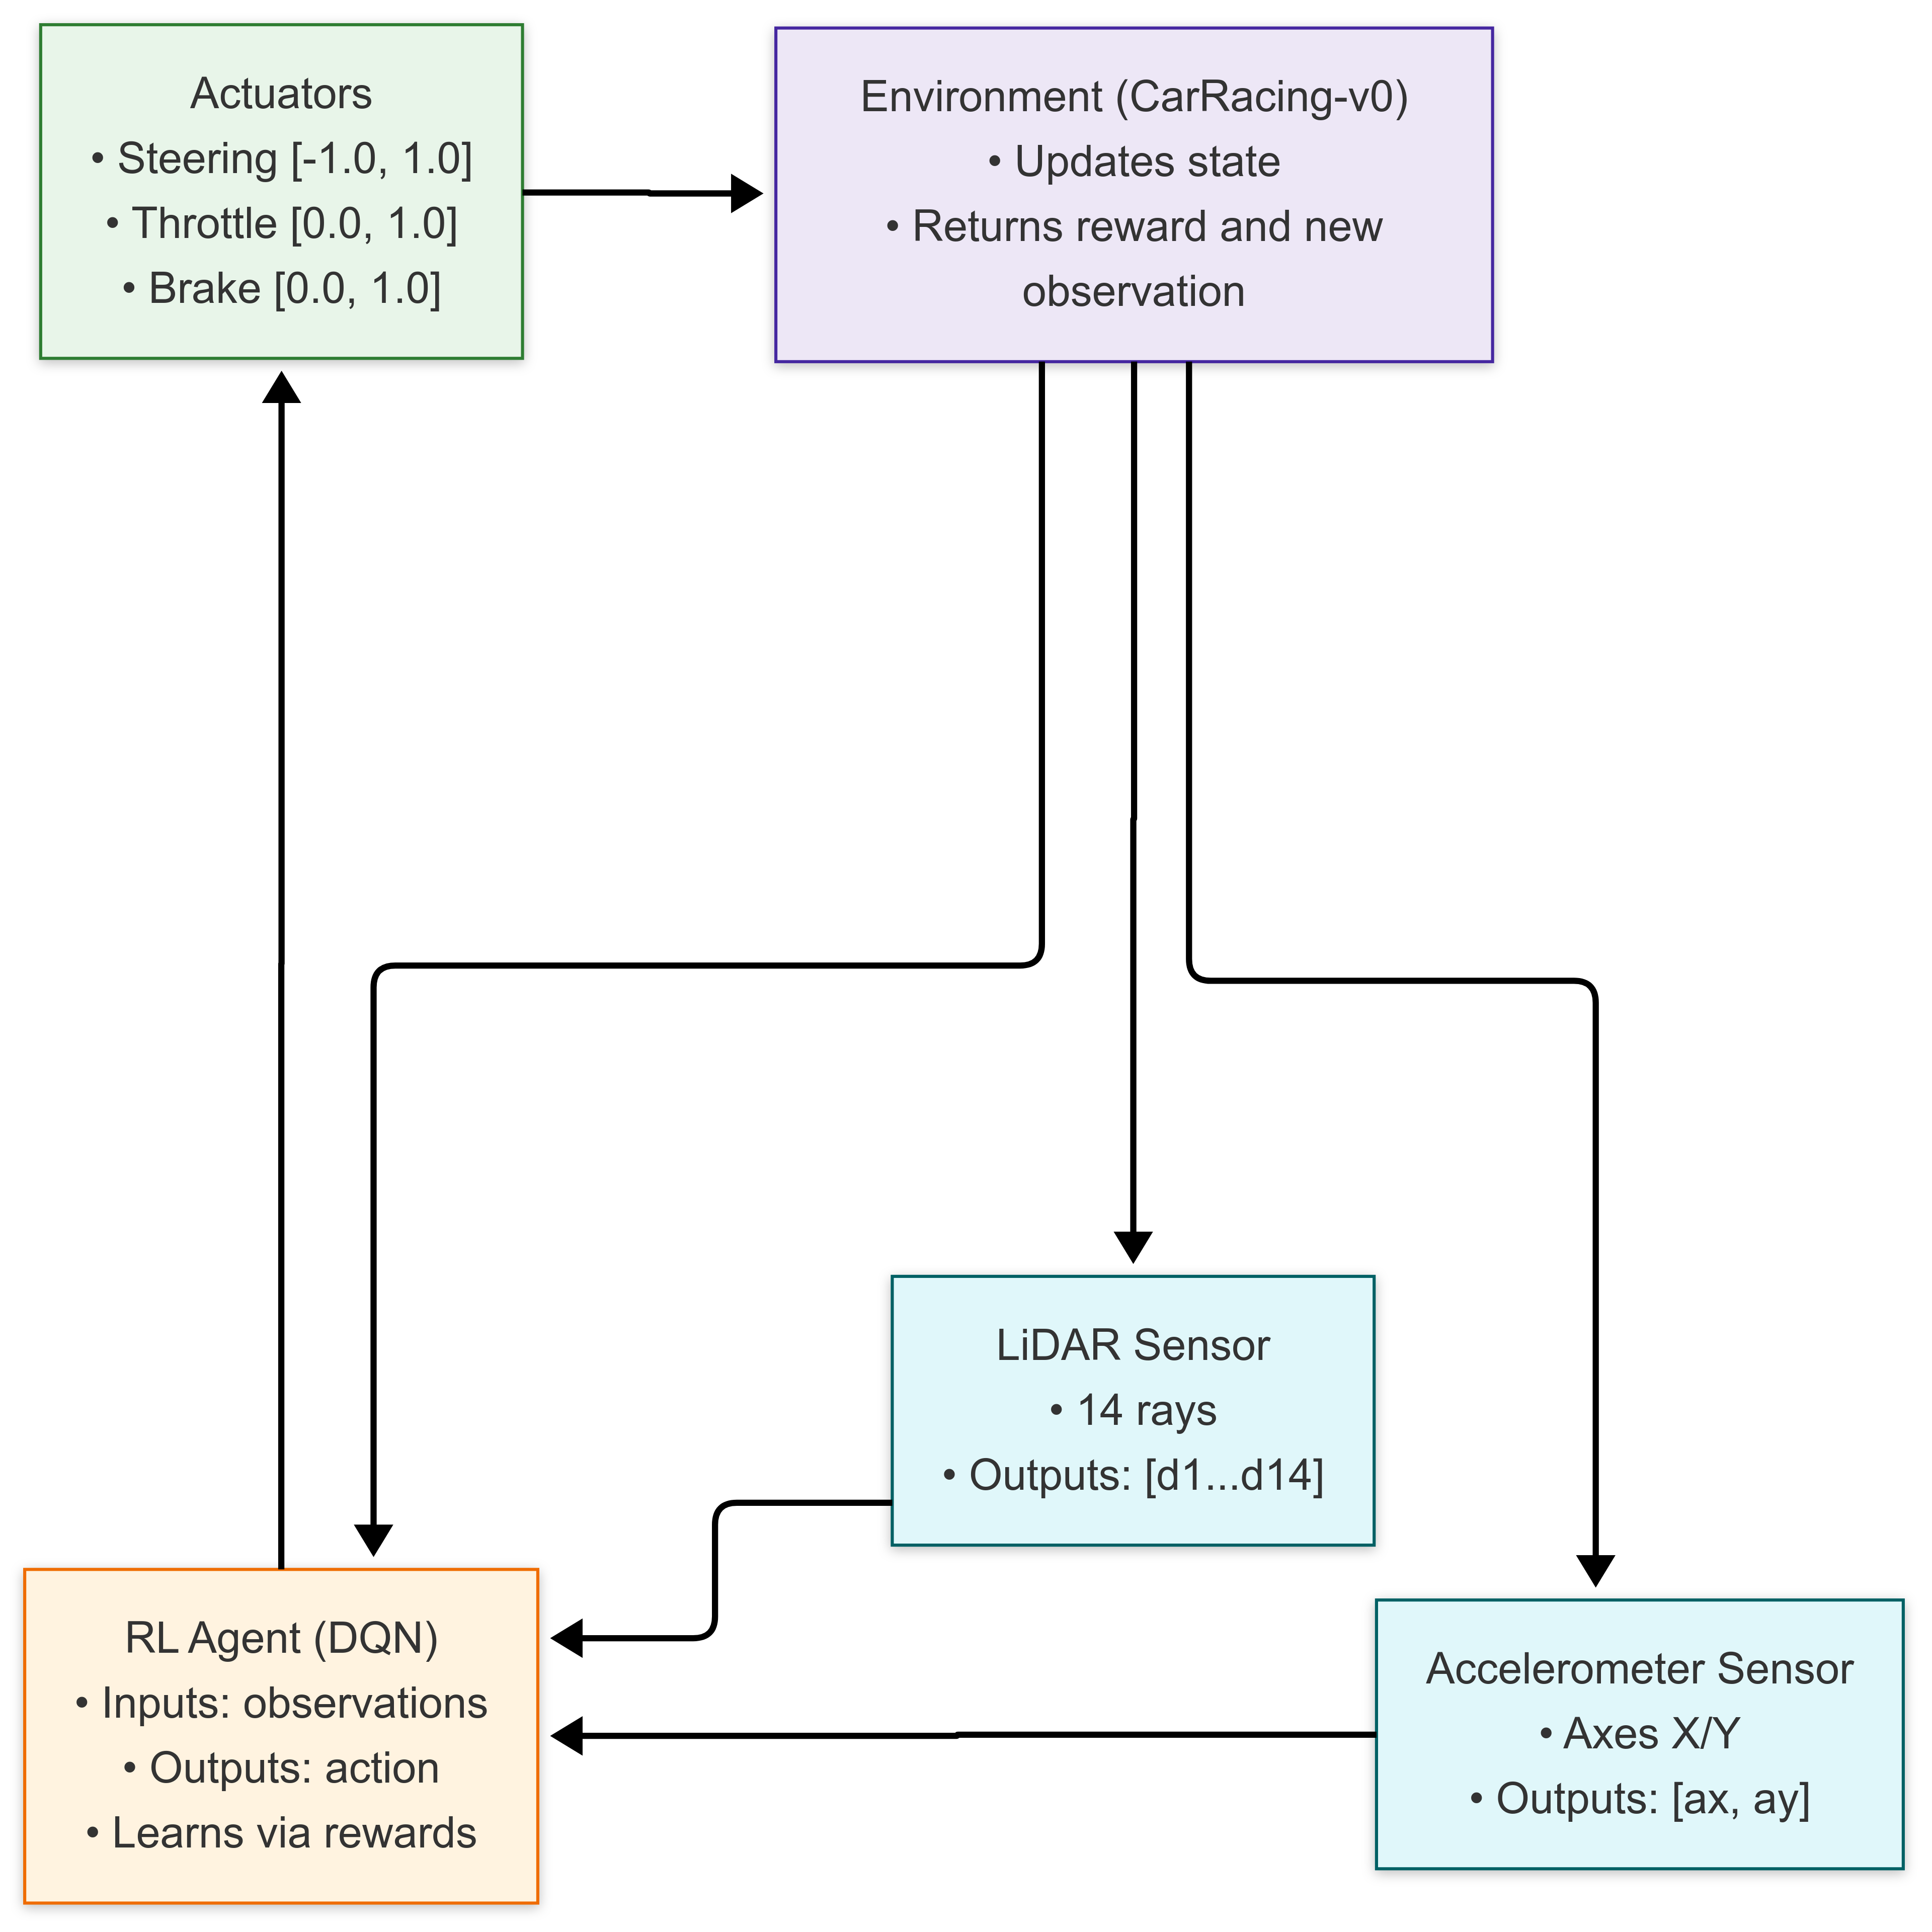
\includegraphics[width=0.8\linewidth]{images/ComponentDiagram.png}
    \caption{Component diagram of the system.}
    \label{fig:component_diagram}
\end{figure}

Our techincal decisions are based on use LiDAR sensors to detect the landmines, and the use of a deep reinforcement learning agent to control the robot. The LiDAR sensors are used to create a 3D map of the environment, and the deep reinforcement learning agent is used to control the robot's movements in the environment. The deep reinforcement learning agent is trained using a reward function that encourages it to move towards the landmines and avoid obstacles. Also we use the giroscope, acceleromenter. The giroscope is used to get the orientation of the robot, the accelerometer is used to get the speed of the robot. The deep reinforcement learning agent is trained using a reward function that encourages it to move towards the landmines and avoid obstacles. The reward function is based on the distance to the landmines and the distance to the obstacles. The deep reinforcement learning agent is trained using a Q-learning algorithm, which is a model-free reinforcement learning algorithm that learns a policy by estimating the value of each action in each state.